\section{SelectionDAG'de RISC-V Tanımı}
\subsection{TableGen Kayıt Bildirimi}
\begin{frame}{TableGen}
    \begin{itemize}
        \item LLVM arka uç tarafında CPP başlık (header) dosyaları oluşturmak için kullanılan alan-özel dili. (Domain specific language/DSL)
        \item
        Talimat bildirim kodundaki fazlalıkları kaldırır
        \item
        Sınıflar, ortak bilgileri aktarmak için kullanılır ve kayıtlara (Records) miras kalır
        \item
        Komutsal (Imperative) yerine Bildirimsel (Declarative)
    \end{itemize}
\end{frame}

\begin{frame}[fragile]{RISC-V TableGen Sınıfları}
Hedef Bağımsız Talimat Sınıfları
    \begin{itemize}
        \item \textbf{InstructionEncoding}, çözücü metodu, talimatın boyutu
        \item
        \textbf{Instruction}, giriş ve çıkış DAG'ları
    \end{itemize}

'XOR' Talimatını bildirmek için Miras Alınan RISC-V Talimat Sınıfları
    \begin{itemize}
        \item \textbf{RVInst}, RISC-V'ın evrensel bit desenleri
        \item
        \textbf{RVInstR}, R tipi talimat
        \item
        \textbf{ALU\_rr}, değişme özelliği (commutativity) gibi özellikler bildirildi
    \end{itemize}
\begin{lstlisting}
def XOR  : ALU_rr<0b0000000, 0b100, "xor", /*Degisebilir*/1>,
           Sched<[WriteIALU, ReadIALU, ReadIALU]>;
\end{lstlisting}
\end{frame}


\subsection{TableGen Desen Eşleştirme}
\begin{frame}[fragile]{TableGen Desenleri}
RISC-V TableGen sınıfları, herhangi bir talimatı daha yapılandırılmış bir şekilde bildirmek için kullanılabilir.
\par
Talimatın DAG deseni, TableGen'in bir Desen bildiriminde ilan edilebilir. NAXOR (NOT AND XOR) talimatı için bu: LLVM IR montaj (assembly) talimatları ve içsel fonksiyonlar (intrinsic functions) DAG yapısında birleştirilir.

\begin{lstlisting}
def : Pat< (xor (and (not GPR:$src1), GPR:$src2), GPR:$src3),
(NAXOR GPR:$src1, GPR:$src2, GPR:$src3)>;
\end{lstlisting}
\end{frame}

        

\begin{frame}[fragile]{TableGen Desenleri}
\begin{lstlisting}
let hasSideEffects = 0, mayLoad = 0, mayStore = 0 in
class ALU_rrr<bits<2> funct2, bits<3> funct3, string opcodestr,
             bit Commutable = 0>
    : RVInstR4<funct2, funct3, OPC_OP, (outs GPR:$rd), (ins GPR:$rs1, GPR:$rs2, GPR:$rs3),
              opcodestr, "$rd, $rs1, $rs2 ,$rs3"> {
  let isCommutable = Commutable;
}
\end{lstlisting}
ALU\_rrr adında özel bir talimat sınıfı oluşturuldu. NAXOR talimatı üç kaynak yazmaç gerektirir ve ALU türü olarak tanımlanır. 
\end{frame}


        
\begin{frame}[fragile]{TableGen Desenleri}
\begin{lstlisting}
def NAXOR     : ALU_rrr<0b11, 0b100, "naxor">,
Sched<[WriteIMul, ReadIMul, ReadIMul]>;
\end{lstlisting}
NAXOR talimatı tanımlanmıştır ve ALU\_rrr talimat türü kullanılmıştır. funct2, funct3, opcode dizesi ve programlar, özel ALU\_rrr sınıfı sayesinde talimatın tam tanımına sahip olmak için yeterlidir.
\end{frame}



\begin{frame}[fragile]{TableGen Desenleri}
\begin{figure}
    \centering
    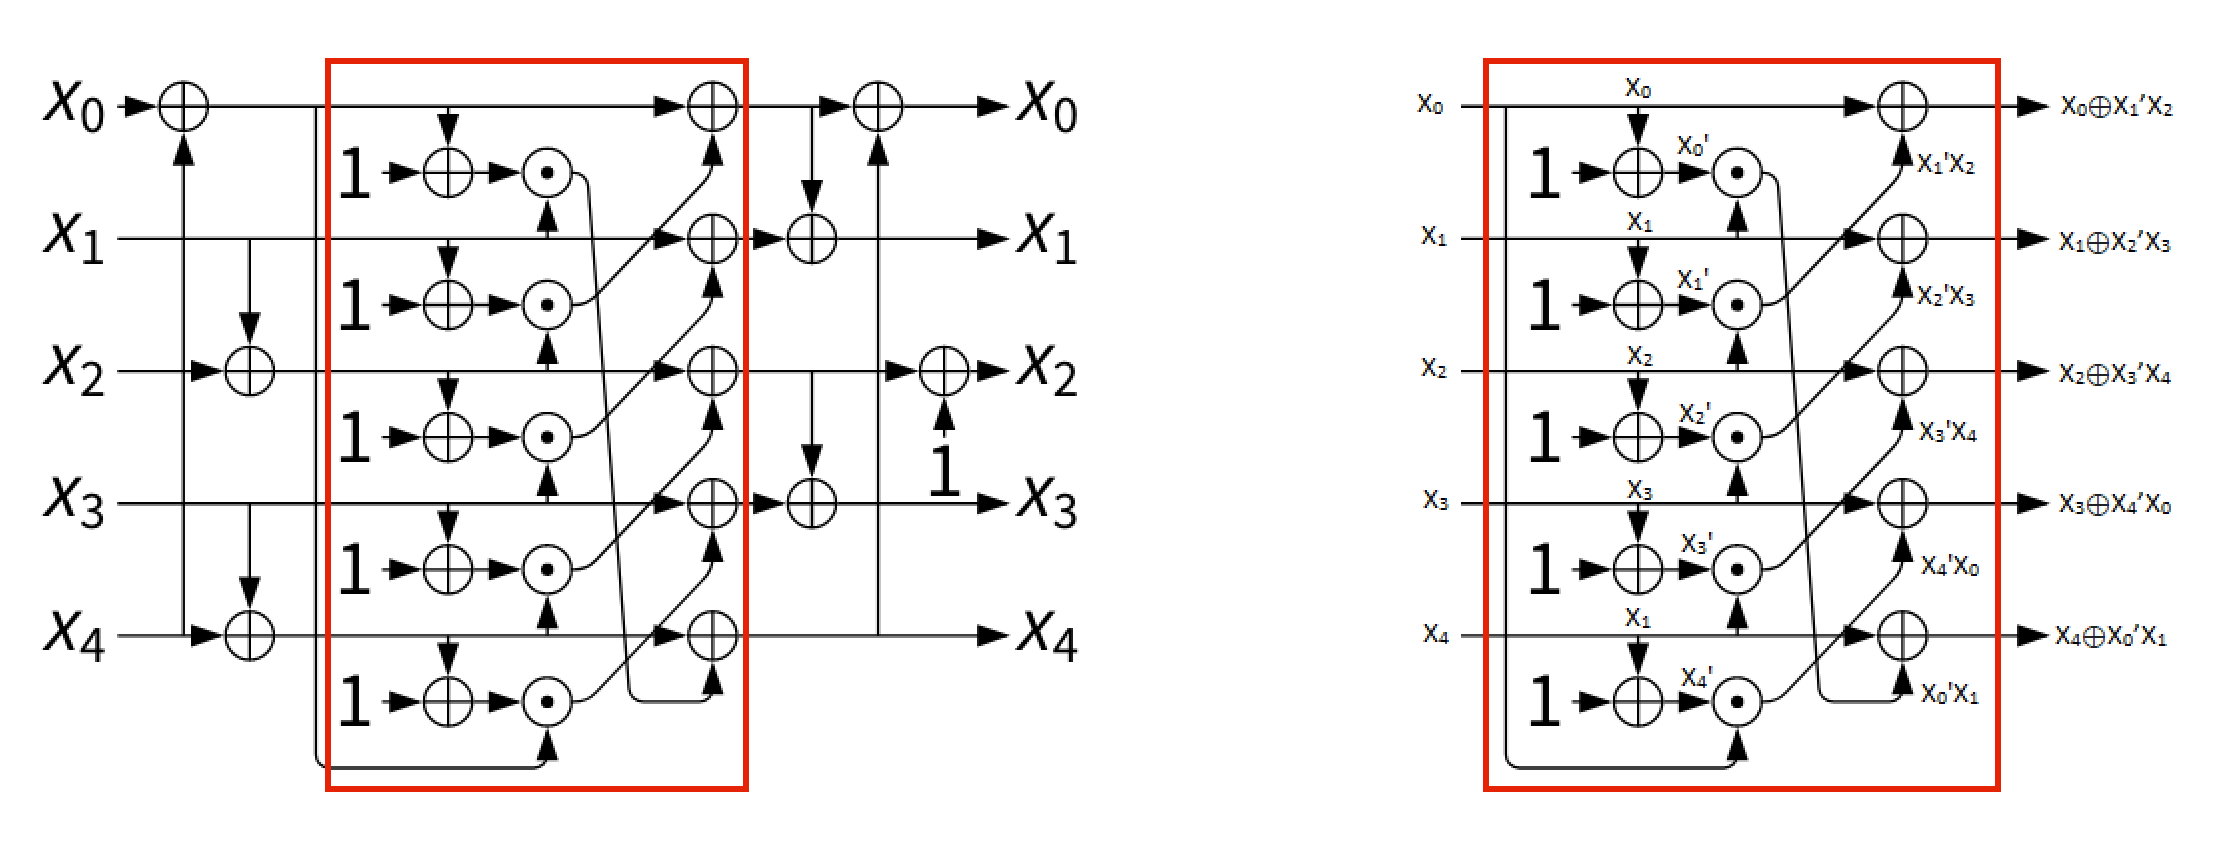
\includegraphics[scale=0.15]{sbox_naxor_pattern.png}
    \caption{NAXOR desenleri s-box algoritmasında}
    \label{fig:sbox_naxor_pattern}
\end{figure}
Bu desen, Şekil \ref{fig:sbox_naxor_pattern}'de vurgulandığı gibi 5 kez tekrarlanır. NAXOR talimatı 15 talimatı 5 talimata indirger.
\end{frame}



\begin{frame}[fragile]{TableGen Desenleri}
\begin{figure}
    \centering
    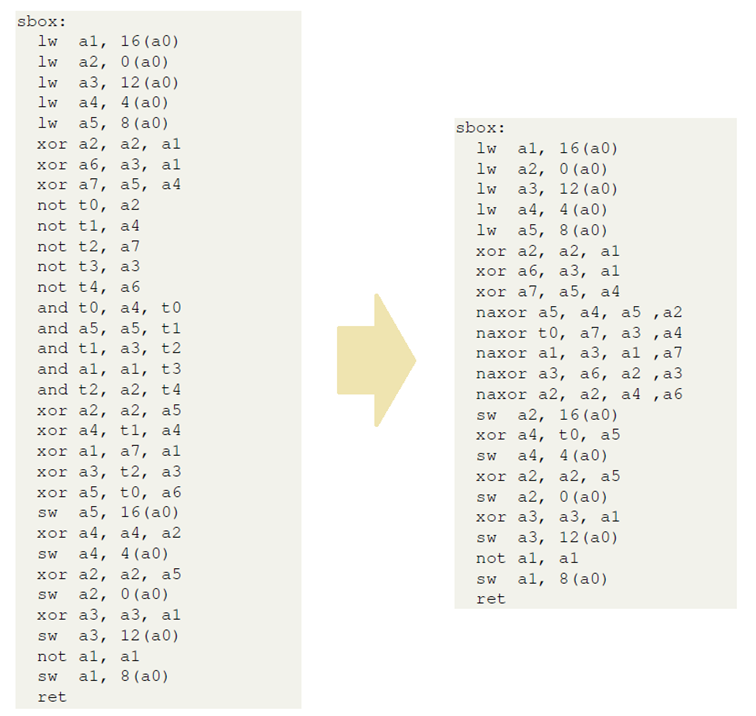
\includegraphics[scale=0.27]{naxor_instruction.png}
    \caption{NAXOR talimatının S-BOX montaj kodu üzerindeki etkisi}
    \label{fig:sbox_instruction}
\end{figure}
S-box algoritması, tekrar tekrar kullanılan belirli bir desen içerir.
NOT-AND-XOR deseni bir s-box döngüsünde beş kez kullanılır. Bu desen, TableGen kullanılarak tek bir talimata indirgenir. Bu desen eşleştikten sonra montaj (assembly) dosyasının 15 satırı tek bir talimata indirgenir.
\end{frame}
